\documentclass[preprint,12pt,aps,pra,showkeys,amsmath,amssymb,superscriptaddress,floatfix]{revtex4-2}
\usepackage[T1]{fontenc}
\usepackage[utf8]{inputenc}
\usepackage{amsmath,amssymb,amsthm,mathtools,mathrsfs}
\usepackage{microtype,booktabs,enumitem}
\usepackage{xcolor,tikz,etoolbox}
\usepackage[skins,breakable]{tcolorbox}
\usepackage{needspace}
% Keep diagram geometry independent of REVTeX preprint body spacing.
\AtBeginEnvironment{tikzpicture}{\linespread{1}\selectfont}
\usetikzlibrary{arrows.meta,positioning,calc,fit,decorations.pathreplacing}
\usepackage{graphicx}
\usepackage{hyperref}

\definecolor{MMBlue}{RGB}{0,82,155}
\definecolor{MMOrange}{RGB}{200,80,0}
\tikzset{
 mmnode/.style={draw=MMBlue,rounded corners=2pt,fill=MMBlue!4,align=left,execute at begin node={\raggedright},text width=5cm,font=\fontsize{10}{12}\selectfont,inner sep=6pt},
 mmimport/.style={mmnode,draw=black!65,fill=black!4},
 mmcandidate/.style={mmnode,draw=MMOrange,dashed,fill=MMOrange!5},
 mmrejected/.style={mmnode,draw=black,densely dotted,fill=black!8},
 mmproof/.style={->,thick,MMBlue},
 mmflow/.style={->,semithick,black!70},
 mmrepair/.style={->,dashed,thick,MMOrange},
 mmcandidatearrow/.style={->,dashed,semithick,MMOrange},
 mmnote/.style={font=\scriptsize,fill=white,inner sep=2pt,align=center}}

\usepackage[section]{placeins}
\setlength{\emergencystretch}{3em}
\setlist{itemsep=3pt,topsep=4pt}
\newtheorem{theorem}{Theorem}[section]
\newtheorem{proposition}[theorem]{Proposition}
\newtheorem{lemma}[theorem]{Lemma}
\newtheorem{corollary}[theorem]{Corollary}
\theoremstyle{definition}
\newtheorem{definition}[theorem]{Definition}
\newtheorem{example}[theorem]{Example}
\theoremstyle{remark}
\newtheorem{remark}[theorem]{Remark}
% Avoid isolated statement headings and single-line paragraph fragments.
\BeforeBeginEnvironment{theorem}{\Needspace{6\baselineskip}}
\BeforeBeginEnvironment{definition}{\Needspace{5\baselineskip}}
\BeforeBeginEnvironment{proposition}{\Needspace{5\baselineskip}}
\BeforeBeginEnvironment{lemma}{\Needspace{5\baselineskip}}
\BeforeBeginEnvironment{corollary}{\Needspace{5\baselineskip}}
\clubpenalty=5000
\widowpenalty=5000
\newcommand{\R}{\mathbb R}\newcommand{\Z}{\mathbb Z}\newcommand{\N}{\mathbb N}
\newcommand{\Pa}{\operatorname{Pa}}\newcommand{\Desc}{\operatorname{Desc}}
\newcommand{\cl}{\operatorname{cl}}\newcommand{\cost}{\operatorname{cost}}
\newcommand{\status}{\operatorname{status}}
% Faculty cards: a visual rail groups the five faculties within one agent.
% The rail has no arrowhead and does not represent a proof dependency.
\newcommand{\mmfacultybadge}[1]{%
 \node[circle,draw=MMBlue,line width=1pt,fill=white,
 minimum size=7mm,inner sep=0pt,font=\sffamily\small\bfseries,text=MMBlue]
 at ([xshift=15pt,yshift=-15pt]frame.north west) {#1};}
\newcommand{\mmfacultyrail}{%
 \draw[MMBlue!80,line width=1pt]
 ([xshift=15pt,yshift=2pt]frame.north west)--
 ([xshift=15pt,yshift=-2pt]frame.south west);}
\newtcolorbox{mmfacultybox}[2]{enhanced,breakable,
 colback=MMBlue!4,colframe=MMBlue!4,boxrule=0pt,arc=3pt,
 left=39pt,right=9pt,top=4pt,bottom=4pt,
 before skip=2pt,after skip=2pt,
 fontupper=\small\linespread{1.1}\selectfont,
 overlay unbroken={\mmfacultyrail\mmfacultybadge{#1}},
 overlay first={\mmfacultyrail\mmfacultybadge{#1}},
 overlay middle={\mmfacultyrail},overlay last={\mmfacultyrail}}
\newcommand{\mmfaculty}[3]{%
 \begin{mmfacultybox}{#1}{#2}
 {\sffamily\bfseries\color{MMBlue}#2}\par\smallskip #3
 \end{mmfacultybox}}
\newcommand{\agent}[9]{%
 \Needspace{8\baselineskip}
 \subsubsection{#1}
 \noindent\textbf{Object.} #2\par
 \noindent\textbf{Role.} #3\par\smallskip
 \mmfaculty{E}{Ego}{#4}
 \mmfaculty{M}{Memory}{#5}
 \mmfaculty{I}{Intellect}{#6}
 \mmfaculty{S}{Sense}{#7}
 \mmfaculty{A}{Action}{#8}
 \smallskip\noindent #9\par}

\usepackage{longtable,array,calc}
\providecommand{\tightlist}{\setlength{\itemsep}{2pt}\setlength{\parskip}{0pt}}
\makeatletter
\def\frontmatter@abstract@produce{\par\addvspace{\frontmatter@preabstractspace}%
\begingroup\prep@absbox\unvbox\absbox\post@absbox\endgroup
\addvspace{\frontmatter@postabstractspace}}
\makeatother
\newcommand{\field}[2]{\par\smallskip\noindent\textbf{#1.} #2\par}
\setlength{\emergencystretch}{5em}
\AtBeginEnvironment{verbatim}{\small\linespread{1.0}\selectfont}


\hypersetup{colorlinks=true,linkcolor=MMBlue,urlcolor=MMBlue,pdfauthor={Dibakar Sigdel}}

\begin{document}

\title{Multivariable Taylor Theorem\\[4pt]\large An End-to-End Meta-Math Walkthrough}

\author{Dibakar Sigdel}

\affiliation{Mindverse Computing LLC, Lynnwood, WA 98087, USA}

\date{October 2026}

\begin{abstract}

A complete authored walkthrough of multivariable taylor theorem, with
explicit mathematical contracts, local verification gates, and reusable
exports. The report presents the target theorem, declared imports, a
dependency graph, five-faculty node contracts, a continuous proof, a
worked example, and a hypothesis-repair audit. It is an authored
mathematical exposition, not a deployed-agent transcript or a formal
proof-assistant certificate.

\end{abstract}\maketitle\linespread{1.12}\selectfont

\noindent\textbf{AC-03 / Advanced Calculus / Report v1}

\section{Target and import contract}

\begin{theorem}

Let \(f:U\subset\mathbb R^n\to\mathbb R\) be \(C^{k+1}\), with the
segment from \(a\) to \(a+h\) in \(U\). Prove
\(f(a+h)=\sum_{j=0}^k D^jf(a)[h,\ldots,h]/j!+\frac1{k!}\int_0^1(1-t)^kD^{k+1}f(a+th)[h,\ldots,h]\,dt\).

\end{theorem}

\subsection{Foundations and permitted imports}

\(D^j\) \(f(a)\) denotes the symmetric j-linear derivative; \(D^0f=f\).
Import the chain rule and AC-02. The segment is contained in open U and
f is \(C^{(k+1)}\) near it, so \(g(t)=f(a+th)\) has the necessary
derivatives on a neighborhood of{[}0,1{]}. Derive the one-variable
integral remainder below.

Here \(k\ge0\) is an integer, \(U\subset\mathbb R^n\) is open, and the
entire segment from \(a\) to \(a+h\) lies in \(U\).

\clearpage\section{Node interaction workflow}

\begin{center}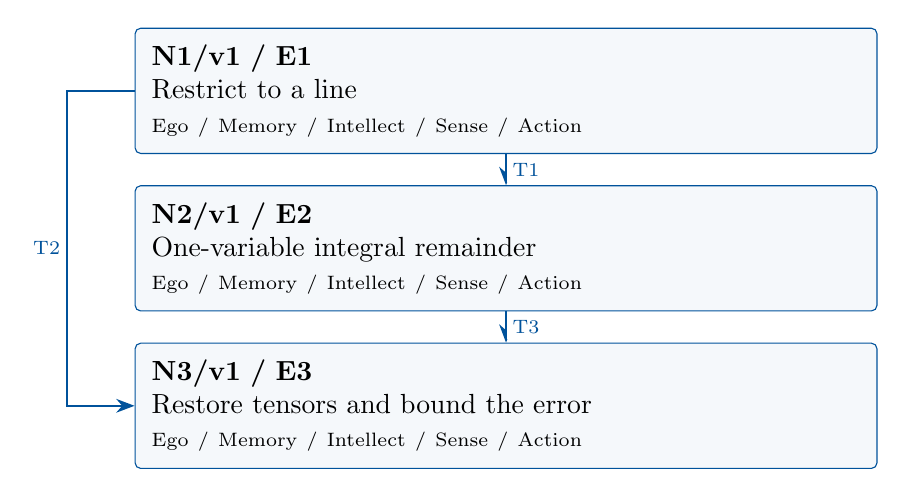
\begin{tikzpicture}[>=Stealth,x=1cm,y=1cm]

\node[mmnode,text width=9cm,minimum height=1.25cm] (N1) at (0,0.0) {\textbf{N1/v1 / E1}\\Restrict to a line\\{\scriptsize Ego / Memory / Intellect / Sense / Action}};

\node[mmnode,text width=9cm,minimum height=1.25cm] (N2) at (0,-2.0) {\textbf{N2/v1 / E2}\\One-variable integral remainder\\{\scriptsize Ego / Memory / Intellect / Sense / Action}};

\node[mmnode,text width=9cm,minimum height=1.25cm] (N3) at (0,-4.0) {\textbf{N3/v1 / E3}\\Restore tensors and bound the error\\{\scriptsize Ego / Memory / Intellect / Sense / Action}};

\draw[mmproof] (N1.south) -- node[mmnote,right] {T1} (N2.north);

\draw[mmproof] (N1.west) -- (-5.58,0) -- node[mmnote,left] {T2} (-5.58,-4) -- (N3.west);

\draw[mmproof] (N2.south) -- node[mmnote,right] {T3} (N3.north);

\end{tikzpicture}\end{center}

Each box is one mathematical agent containing all five faculties. Blue
arrows carry the versioned exports listed below. The layout gives a
reading order; only drawn arrows assert dependencies. Diagnostic repair
is separate from the proof DAG.

\subsection{Versioned evidence-transfer ledger}

\begingroup\small\linespread{1.05}\selectfont

\Needspace{5\baselineskip}\field{T1: N1/E1/v1 to N2}{The directional derivative identities along the entire segment.}

\field{Receiving activity}{N2: One-variable integral remainder}

\field{Compatibility}{Use the same mathematical objects and hypotheses as the source export.
Receiving contract: \(g\in C^{(k+1)}\) near{[}0,1{]}; prior exports
E1/v1}

\Needspace{5\baselineskip}\field{T2: N1/E1/v1 to N3}{The directional derivative identities along the entire segment.}

\field{Receiving activity}{N3: Restore tensors and bound the error}

\field{Compatibility}{Use the same mathematical objects and hypotheses as the source export.
Receiving contract: Directional identities and scalar formula; prior
exports E1/v1, E2/v1}

\Needspace{5\baselineskip}\field{T3: N2/E2/v1 to N3}{The exact one-variable Taylor formula with integral remainder.}

\field{Receiving activity}{N3: Restore tensors and bound the error}

\field{Compatibility}{Use the same mathematical objects and hypotheses as the source export.
Receiving contract: Directional identities and scalar formula; prior
exports E1/v1, E2/v1}

\endgroup

\clearpage\section{Agent roles and five-faculty activities}\begingroup\small\linespread{1.05}\selectfont\setlist{itemsep=1pt,topsep=2pt}

\subsection{N1/v1: Restrict to a line}

\field{Object and role}{Reduce the multivariable increment to a scalar parameter.}

\field{Inputs}{\(f\in C^{(k+1)}\); \(a+th\in U\) for \(0\le t\le 1\); foundational
imports stated in §1}

\mmfaculty{E}{Ego}{Own E1/v1: The directional derivative identities along the entire
segment.}

\mmfaculty{M}{Memory}{Retain \(f\in C^{(k+1)}\); \(a+th\in U\) for \(0\le t\le 1\);
foundational imports stated in §1; keep their assumptions and versions
attached.}

\mmfaculty{I}{Intellect}{Reduce the multivariable increment to a scalar parameter.}

\mmfaculty{S}{Sense}{Endpoint-only domain membership is insufficient if the segment leaves U.}

\mmfaculty{A}{Action}{Carry out the numbered deductions and publish E1/v1 together with its
hypotheses and proof location.}

\smallskip\noindent\textbf{Numbered mathematical activities}

\begin{enumerate}[label=N1.\arabic*,leftmargin=3.4em]

\item Define \(g(t)=f(a+th)\).

\item Repeated chain rule along the affine path yields
\(g^{(j)}(t)=D^jf(a+th)[h,\ldots ,h]\) for \(0\le j\le k+1\).

\item For \(j=0\) this means the function itself.

\item Compactness of the segment gives a neighborhood on which these
restrictions are defined; no global convexity of U is assumed.

\end{enumerate}

\field{Export E1/v1}{The directional derivative identities along the entire segment.}

\field{Acceptance gate}{Endpoint-only domain membership is insufficient if the segment leaves U.
Publish only after checking every displayed deduction.}

\field{Targeted repair}{If the check fails, revise N1: Endpoint-only domain membership is
insufficient if the segment leaves U. Recheck dependent nodes N2, N3.}

\clearpage

\subsection{N2/v1: One-variable integral remainder}

\field{Object and role}{Apply FTC and integrate by parts repeatedly.}

\field{Inputs}{\(g\in C^{(k+1)}\) near{[}0,1{]}; prior exports E1/v1}

\mmfaculty{E}{Ego}{Own E2/v1: The exact one-variable Taylor formula with integral
remainder.}

\mmfaculty{M}{Memory}{Retain \(g\in C^{(k+1)}\) near{[}0,1{]}; prior exports E1/v1; keep their
assumptions and versions attached.}

\mmfaculty{I}{Intellect}{Apply FTC and integrate by parts repeatedly.}

\mmfaculty{S}{Sense}{The factorial and sign follow from the integration-by-parts recursion.}

\mmfaculty{A}{Action}{Carry out the numbered deductions and publish E2/v1 together with its
hypotheses and proof location.}

\smallskip\noindent\textbf{Numbered mathematical activities}

\begin{enumerate}[label=N2.\arabic*,leftmargin=3.4em]

\item For \(k=0\), \(g(1)-g(0)=\int _{0}^{1}g'(t)dt\) by FTC.

\item For \(k\ge 1\) integrate \(I_k=(1/k!)\int _{0}^{1}(1-t)^k\)
\(g^{(k+1)}(t)dt\) by parts.

\item The upper boundary is 0, the lower boundary contributes
\(-g^{(k)}(0)/k!\), and the remaining integral is \(I_{k-1}\).

\item Hence \(I_k=I_{k-1}-g^{(k)}(0)/k!\).

\item Iterating to \(I_{0}=g(1)-g(0)\) gives \(g(1)=\sum _{j=0}^k\)
\(g^{(j)}(0)/j!+I_k\).

\end{enumerate}

\field{Export E2/v1}{The exact one-variable Taylor formula with integral remainder.}

\field{Acceptance gate}{The factorial and sign follow from the integration-by-parts recursion.
Publish only after checking every displayed deduction.}

\field{Targeted repair}{If the check fails, revise N2: The factorial and sign follow from the
integration-by-parts recursion. Recheck dependent nodes N3.}

\clearpage

\subsection{N3/v1: Restore tensors and bound the error}

\field{Object and role}{Keep all k+1 factors of h in the remainder.}

\field{Inputs}{Directional identities and scalar formula; prior exports E1/v1, E2/v1}

\mmfaculty{E}{Ego}{Own E3/v1: Exact tensor expansion and a certified norm remainder bound.}

\mmfaculty{M}{Memory}{Retain Directional identities and scalar formula; prior exports E1/v1,
E2/v1; keep their assumptions and versions attached.}

\mmfaculty{I}{Intellect}{Keep all k+1 factors of h in the remainder.}

\mmfaculty{S}{Sense}{A scalar Hessian expression must not omit mixed terms or directional
factors.}

\mmfaculty{A}{Action}{Carry out the numbered deductions and publish E3/v1 together with its
hypotheses and proof location.}

\smallskip\noindent\textbf{Numbered mathematical activities}

\begin{enumerate}[label=N3.\arabic*,leftmargin=3.4em]

\item Substitute the node1 derivative identities into the formula to obtain
exactly the asserted expansion for \(f(a+h)\).

\item If L bounds the operator norm of \(D^{(k+1)}f\) on the segment, the
remainder has modulus at most \(L\Vert h\Vert ^{(k+1)}/k!\) times
\(\int _{0}^{1}(1-t)^kdt=L\Vert h\Vert ^{(k+1)}/(k+1)!\).

\item The bound is an additional reusable estimate with its explicit L; if
\(h=0\) all positive-order terms and the remainder vanish.

\end{enumerate}

\field{Export E3/v1}{Exact tensor expansion and a certified norm remainder bound.}

\field{Acceptance gate}{A scalar Hessian expression must not omit mixed terms or directional
factors. Publish only after checking every displayed deduction.}

\field{Targeted repair}{If the check fails, revise N3: A scalar Hessian expression must not omit
mixed terms or directional factors. Withhold this terminal result until
its gate passes.}

\endgroup\clearpage\section{Continuous mathematical proof}\label{sec:proof}

Read these steps in order as one proof; the diagram is optional.
Numbered activities identify the specific constructions and deductions
owned by each node.

\subsection{§4.N1 --- Restrict to a line}\label{n1-restrict-to-a-line}

\begin{enumerate}
\def\labelenumi{\arabic{enumi}.}
\item
  Define \(g(t)=f(a+th)\).
\item
  Repeated chain rule along the affine path yields
  \(g^{(j)}(t)=D^jf(a+th)[h,\ldots ,h]\) for \(0\le j\le k+1\).
\item
  For \(j=0\) this means the function itself.
\item
  Compactness of the segment gives a neighborhood on which these
  restrictions are defined; no global convexity of U is assumed.
\end{enumerate}

\subsection{§4.N2 --- One-variable integral
remainder}\label{n2-one-variable-integral-remainder}

\begin{enumerate}
\def\labelenumi{\arabic{enumi}.}
\item
  For \(k=0\), \(g(1)-g(0)=\int _{0}^{1}g'(t)dt\) by FTC.
\item
  For \(k\ge 1\) integrate \(I_k=(1/k!)\int _{0}^{1}(1-t)^k\)
  \(g^{(k+1)}(t)dt\) by parts.
\item
  The upper boundary is 0, the lower boundary contributes
  \(-g^{(k)}(0)/k!\), and the remaining integral is \(I_{k-1}\).
\item
  Hence \(I_k=I_{k-1}-g^{(k)}(0)/k!\).
\item
  Iterating to \(I_{0}=g(1)-g(0)\) gives \(g(1)=\sum _{j=0}^k\)
  \(g^{(j)}(0)/j!+I_k\).
\end{enumerate}

\subsection{§4.N3 --- Restore tensors and bound the
error}\label{n3-restore-tensors-and-bound-the-error}

\begin{enumerate}
\def\labelenumi{\arabic{enumi}.}
\item
  Substitute the node1 derivative identities into the formula to obtain
  exactly the asserted expansion for \(f(a+h)\).
\item
  If L bounds the operator norm of \(D^{(k+1)}f\) on the segment, the
  remainder has modulus at most \(L\Vert h\Vert ^{(k+1)}/k!\) times
  \(\int _{0}^{1}(1-t)^kdt=L\Vert h\Vert ^{(k+1)}/(k+1)!\).
\item
  The bound is an additional reusable estimate with its explicit L; if
  \(h=0\) all positive-order terms and the remainder vanish.
\end{enumerate}

\hfill$\square$

\section{Worked orchestration}

For \(f(x,y)=e^{(x+y)}\) at \(a=(0,0)\), \(h=(u,v)\), \(k=1\),
\(Df(a)[h]=u+v\) and \(D^{2}f(th)[h,h]=e^(t(u+v))(u+v)^{2}\). Hence
\(e^{(u+v)}=1+u+v+(u+v)^{2}\int _{0}^{1}(1-t)e^(t(u+v))dt\). The
remainder is at most \(e^|u+v|(u+v)^{2}/2\).

\subsection{Boundary and hypothesis audit}

A first-order Taylor polynomial is generally not an exact value:
\(f(x)=x^{2}\) at 0 has zero first-order polynomial but remainder
\(h^{2}\). Sense requires the integral or a bound instead of dropping
it. The theorem also cannot traverse a missing segment through a hole in
U.

\section{Illustrative failure and repair}

The following is an authored diagnostic scenario. Changed assumptions
define a new contract; they do not retroactively prove the original
statement.

\subsection{Failure and correction}
This is an authored teaching trace, not a recorded agent run.

\begin{enumerate}
\def\labelenumi{\arabic{enumi}.}
\tightlist
\item
  \textbf{Ego \(\to\) Memory:} register the §1 theorem, imports, and
  requested exports before beginning the proof.
\item
  \textbf{Intellect \(\to\) Action:} choose the bridges in §3 and carry
  out the numbered activities in §4; transmit only established E-exports
  along the §2 DAG.
\item
  \textbf{Sense \(\to\) responsible node:} test the specific
  boundary/failure in §5 and the node's individual audit. A failing
  candidate is withheld; downstream nodes may not use it.
\item
  \textbf{Memory + Intellect:} identify whether the error is an omitted
  condition, an invalid inference, or an attempted extension beyond the
  theorem. Restore the exact contract or explicitly state a different
  one.
\item
  \textbf{Action:} redo the affected mathematical activity using the
  repaired condition or inference. Recheck consuming nodes, rather than
  feeding their conclusions back as premises.
\item
  \textbf{Ego:} publish only the supported export with its assumptions
  and proof location. A hypothetical revised export is v2; the written
  proof here is the v1 exposition, not a claim that this repair was
  executed.
\end{enumerate}

\subsection{Hypothesis boundary}
A first-order Taylor polynomial is generally not an exact value:
\(f(x)=x^{2}\) at 0 has zero first-order polynomial but remainder
\(h^{2}\). Sense requires the integral or a bound instead of dropping
it. The theorem also cannot traverse a missing segment through a hole in
U.

\subsection{Version and recheck}
Treat any changed assumption as a new contract. Recheck the revised
export and all of its descendants. A backward diagnostic never
establishes an earlier theorem. This is an authored teaching trace, not
an execution log.

\par\medskip\begingroup\small\linespread{1.0}\selectfont\noindent\textbf{Provenance.} This authored proof is complete relative to its declared imports. Reuse
each export with its assumptions, proof, and version. The original
Markdown remains available for comparison.
\par\endgroup

\end{document}
